\section{Multiple logistic regression models}\label{sec:logist-mult}
The logistic regression model can be generalized to include an
arbitrary number of explanatory variables,
\begin{eqnarray}
  \logit ( \pi_{i})
   &=& \alpha + \vec{x}_{i}\trans \,  \vec{\beta} \\ \label{eq:logisr}
   &=& \alpha + \beta_1 x_{i1} + \beta_2 x_{i2} + \cdots + \beta_p x_{ip}
   \nonumber
\end{eqnarray}
The $x$s can include any of the following sorts of regressors,
as in the general linear model:

\begin{itemize*}
\item \textbf{quantitative} variables (e.g., age, income)
\item \textbf{polynomial} powers of quantitative variables (e.g., age, age$^2$, age$^3$)
\item \textbf{transformations} of quantitative variables (e.g., log salary)
\item \textbf{dummy} variables, representing qualitative predictors (e.g.,
$P_1, P_2, P_3$ for four political party affiliations)
\item \textbf{interaction} terms (e.g., sex $\times$ age, or age $\times$ income)
\end{itemize*}
Again, all the regressors in the model must be created explicitly in
a \Dstp\ for \PROC{LOGISTIC}.

\begin{Example}[arthrit10]{Arthritis treatment}
We now combine the analysis of age (\exref{ex:arthrit7}) with that of
sex and treatment (\exref{ex:arthrit8}) in the
arthritis data.

The DATA step below creates a SAS \Dset\ named \pname{arthrit}, in
case form.  Programming statements are used to
create dummy variables \verb|_sex_| and \verb|_treat_| as before.
Variables for testing interactions among sex, treatment and age
are also created.  A preliminary analysis (described in \exref{ex:arthrit11}) is used
to test whether any of these variables interact.  That test shows
that all interactions can safely be ignored in this example.  That
test also serves as a 
goodness of fit test for the main effects
model treated here.
\begin{output}
data arthrit;
   length treat$7. sex$6. ;
   input id treat$ sex$ age improve @@ ;
   better  = (improve > 0);            /* Dichotomous response    */
   _treat_ = (treat ='Treated') ;      /* Dummy var for treatment */
   _sex_   = (sex = 'Female');         /*           and sex       */
   agesex  = age*_sex_ ;               /* Dummy var for testing   */
   agetrt  = age*_treat_;              /*   interactions          */
   sextrt  = _sex_*_treat_;
   age2    = age*age ;
 datalines ;
57 Treated Male   27 1   9 Placebo Male   37 0
46 Treated Male   29 0  14 Placebo Male   44 0
77 Treated Male   30 0  73 Placebo Male   50 0
  ... {\it (observations omitted)}
56 Treated Female 69 1  42 Placebo Female 66 0
43 Treated Female 70 1  15 Placebo Female 66 1
                        71 Placebo Female 68 1
                         1 Placebo Female 74 2
\end{output}
The next logistic model includes (main) effects for age, sex, and
treatment. In this example, we
plot both a confidence interval for Pr\{Improved\} and for the \(\logit
\pm  1\mbox{s.e.}\).  To make these intervals roughly comparable, we
choose \(\alpha  = .33\) to give a 67\%  confidence interval.

\begin{listing}
title2 'Estimated Effects of Age, Treatment and Sex';
proc logistic data=arthrit;
   format better outcome.;
   model  better = _sex_  _treat_  age / lackfit;
   output out=results p=predict l=lower u=upper
                      xbeta=logit stdxbeta=selogit / alpha=.33;
\end{listing}
The printed results are shown in \outref{out:glogist1.1}.
The parameter values are similar to those in the earlier examples,
and have the same interpretations.
For example, for age, the odds ratio of 1.050
means that the odds of improvement increases 5\% per year.
Over 10 years, the odds of improvement would be multiplied by \(e^{.487} = 1.63\), a 63\% increase.

\begin{Output}[htb]
\caption{Arthritis data: Overall tests and parameter estimates}\label{out:glogist1.1}
\small
\verbatiminput{ch6/out/glogist1.1}
\end{Output}

Plots are constructed from the \Dset\ RESULTS.  The first few
observations are shown below.

\begin{output}
   ID   TREAT   AGE   SEX  IMPROVE  PREDICT   LOWER   UPPER   LOGIT SELOGIT

   57  Treated   27  Male     1       0.194   0.103   0.334  -1.427   0.758
    9  Placebo   37  Male     0       0.063   0.032   0.120  -2.700   0.725
   46  Treated   29  Male     0       0.209   0.115   0.350  -1.330   0.728
   14  Placebo   44  Male     0       0.086   0.047   0.152  -2.358   0.658
     ...
\end{output}


%% two subfig side-by-side
\begin{figure}[htb]
 \begin{minipage}[t]{.49\linewidth}
  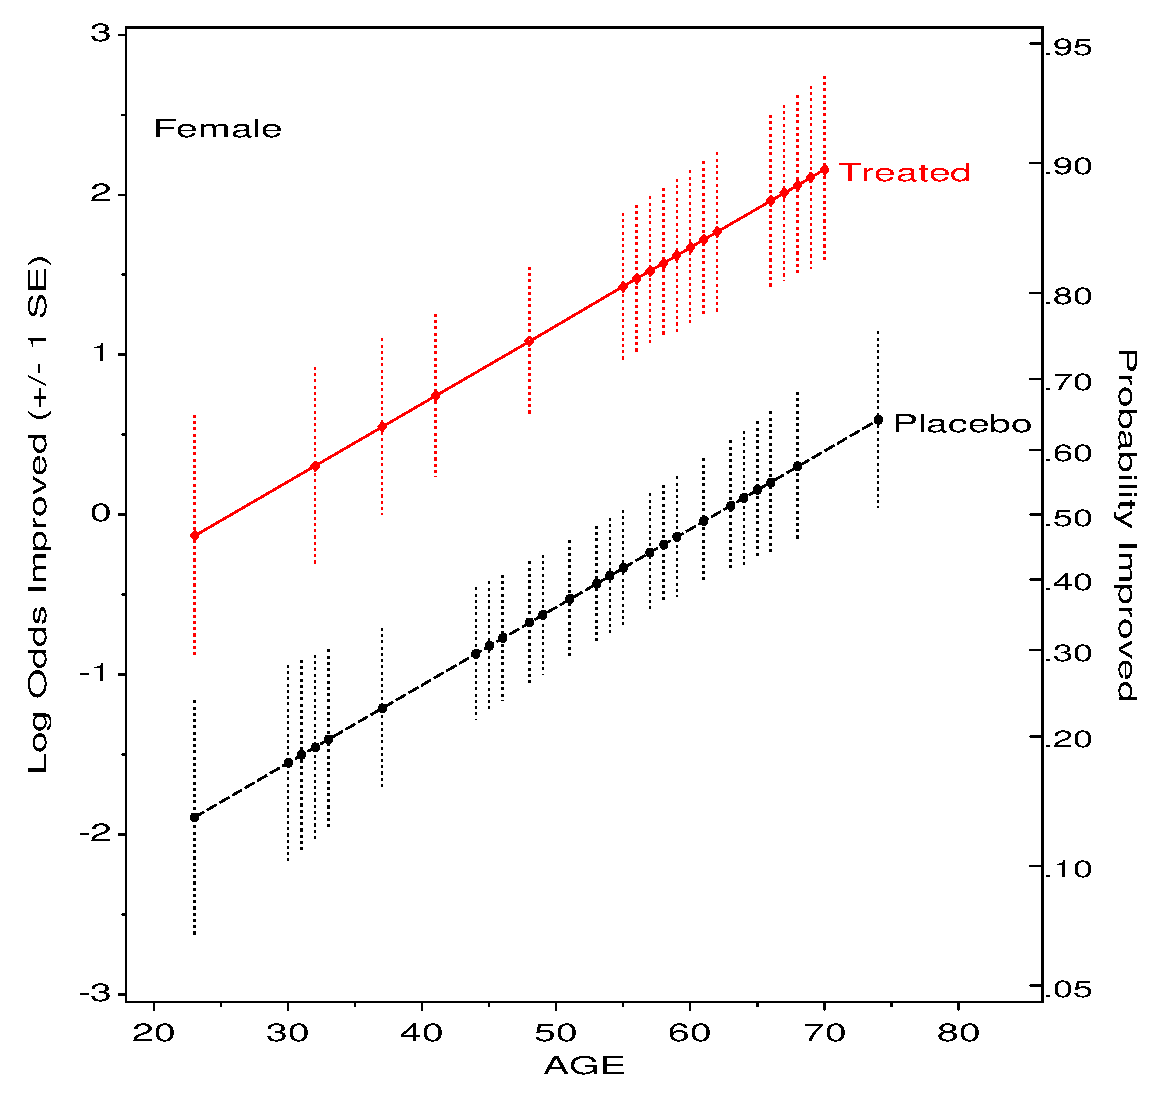
\includegraphics[width=1\linewidth]{ch6/fig/glogist1b1}
 \end{minipage}%
 \hfill
 \begin{minipage}[t]{.49\linewidth}
  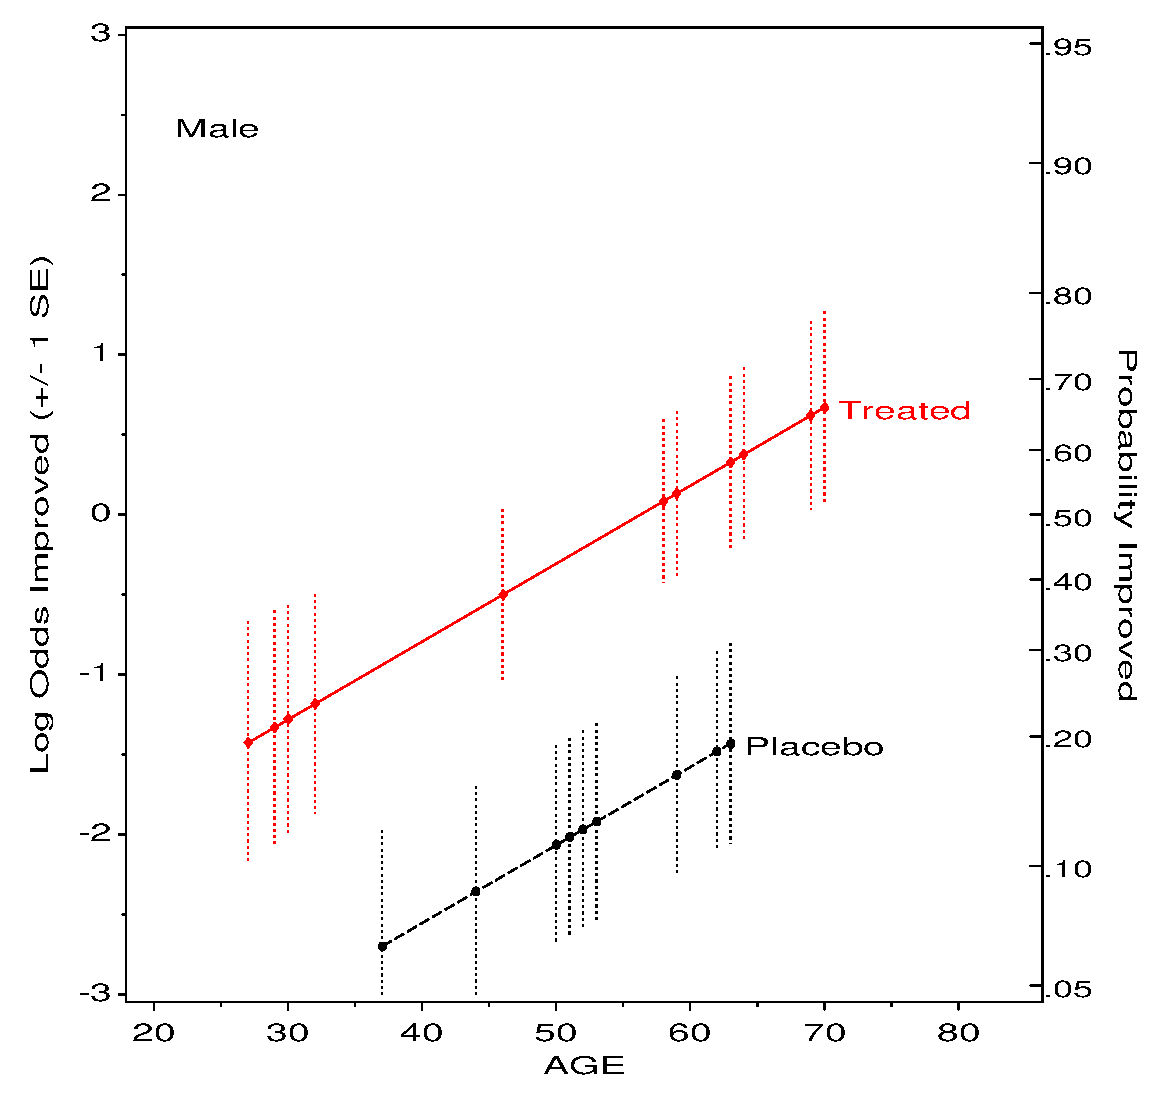
\includegraphics[width=1\linewidth]{ch6/fig/glogist1b2}
 \end{minipage}
 \caption[Estimated logits for sex, treatment and age]{Estimated logits for sex, treatment and age.
 Corresponding probabilities of a ``better'' response are shown on the right scale.}\label{fig:glogist1b}
\end{figure}

Predicted probabilities and confidence limits are contained in the
variables \texttt{PREDICT}, \texttt{UPPER}, and \texttt{LOWER}.
Corresponding logit values and their standard errors
are contained in the variables \texttt{LOGIT} and \texttt{SELOGIT}.
The predicted relations are linear and additive on the logit 
(log odds) scale
according to the model \eqref{eq:logisr},
but perhaps more interpretable on the probability scale.
One reasonable compromise is to plot the predicted log odds
along with an auxiliary scale showing the equivalent probability
values.

To show the
effects of sex, treatment, and age 
on improvement (Pr\{Better\}), 
separate plots
are drawn for each sex, using the statement \texttt{BY SEX;} in a 
\PROC{GPLOT} step.
These are shown side-by-side in \figref{fig:glogist1b},
facilitating their comparison.


Most of the work consists of drawing the confidence
limits with the Annotate facility, but this is worthwhile because it shows
the locations and bounds for individual observations.  
Plots of the predicted probabilities can
be made in a similar way using the variables
\texttt{PREDICT}, \texttt{UPPER}, and \texttt{LOWER}.

%% input: /Users/friendly/sasuser/catdata/glogist1b.sas
%% last modified: 27-Jul-99 15:36
\begin{listing}
proc sort data=results;
   by sex treat age;

data bars;
   set results(keep=sex treat age logit selogit);
   by sex treat;
   length text $8;
   xsys='2'; ysys='2';
   if treat='Placebo' then color='BLACK';
                      else color='RED';
   x  = age; line=33;
   y  = logit+selogit;  function='MOVE   '; output;
   y  = logit-selogit;
   y  = max(-3,y);      function='DRAW   '; output;
   if last.treat then do;
      y = logit;
      x = age+1; position='6';
      text = treat; function='LABEL'; output;
      end;
   if first.sex then do;
      ysys ='1'; y=90;
      xsys ='1'; x=10;
      text = sex; function='LABEL'; output;
      end;
\end{listing}

The probability scale is constructed using the \macro{PSCALE},
which produces an \ADS\ to draw the tick marks and probability
values along the right axis.  The axis label is drawn with a
\stmt{TITLE}{GPLOT} which specifies \pname{ANGLE=-90}.

%% input: /Users/friendly/sasuser/catdata/glogist1b.sas
%% last modified: 28-Jul-99 10:25
\begin{listing}
%pscale(anno=pscale);
data pscale;
   set pscale;
   sex = 'Female'; output;
   sex = 'Male  '; output;
proc sort;
   by sex;
data bars;
   set bars pscale;
   by sex;

title ' '
   h=1.5 a=-90 'Probability Improved'
   h=3.5 a=-90 ' ';
goptions hby=0;
proc gplot data=results;
   plot logit * age = treat / vaxis=axis1 haxis=axis2 hm=1 vm=1
                              nolegend anno=bars frame;
   by sex;
   axis1 label=(a=90 'Log Odds Improved (+/- 1 SE)')
         order=(-3 to 3);
   axis2 order=(20 to 80 by 10) offset=(2,6);
   symbol1 v=+ i=join l=3 c=black;
   symbol2 v=$ i=join l=1 c=red;
run;
\end{listing}

\figref{fig:glogist1b} provides a clear interpretation for the
predicted effects of age combined with those of treatment and
sex that we saw earlier.  On the logit scale, improvement increases
linearly with age.  The probability scale allows us to understand
the predicted values more readily.   For instance, we can see that
50 year-old woman given the active treatment
has a predicted probability of improvement
around 0.80, but a probability less than 0.40 if given the placebo.

Because the model includes no interaction terms, the fitted lines
are parallel for all treatment--sex groups, and the effects of all
variables are large compared to their standard errors.
However, we are only plotting fitted values here and should be
cautious until we have tested for interactions among these variables.
We do this in \secref{sec:logist-multint} (\exref{ex:arthrit11}).
\end{Example}
\begin{Example}[icu1]{Survival in the ICU}
In this example we examine briefly some aspects of logistic regression
related to model selection and graphical display with a mixture of
quantitative and discrete variables.
We use data from a study by
\citet{Lemeshow-etal:88}
of patients admitted to an intensive care unit at
Baystate Medical Center in Springfield,
Massachusetts.  The goal of this study was to develop a
model to predict the probability of survival (up to hospital
discharge) of these patients and to study the risk factors associated with 
ICU mortality.
Data for a sample of 200 subjects from this study are given in
\citet[App. 2]{HosmerLemeshow:89}, and reproduced in
\datref{dat:icu}.

There are 19 explanatory variables, of which three (age, systolic blood pressure and heart rate) are quantitative, one is categorical (race),
and the remaining 15 are binary (many having been dichotomized).
Initial model screening was carried out using the forward, backward,
and stepwise procedures using the \opt{SELECTION}{LOGISTIC}
on the \stmt{MODEL}{LOGISTIC}.  As in other model selection procedures,
it is prudent to regard these simply as ``candidate'' models,
nominated for further attention. 
The results for the full model with
all 19 predictors and for the final selection models are shown below.

\begin{center}
 \begin{tabular}{l rrrrr p{5.5cm}}
 \hline
  Selection & AIC & SC & $G^2$ & Score & df & Variables in Model \\ 
  \hline
  Full model & 160.78 & 226.74 & 79.38 & 74.74 & 19 & All \\ 
  Stepwise & 149.14 & 165.63 & 61.03 & 62.67 & 4 & Age Cancer Admit Uncons \\ 
  Forward & 149.14 & 165.63 & 61.03 & 62.67 & 4 & Age Cancer Admit Uncons \\ 
  Backward & 144.44 & 170.83 & 71.72 & 70.52 & 7 & Age Cancer Admit Uncons Systolic pH PCO \\ 
 \hline
 \end{tabular}
\end{center}

For the moment, we focus on the variables Age, Cancer, Admit
(elective vs.\ emergency admission) and
Uncons
(stupor or coma at admission).  These were nominated by all three procedures, and 
constitute the best model according to the forward and stepwise
procedures.  Estimated coefficients and odds ratios for this model
are shown in \outref{out:icu1.1}, fit using the statements below.
The lack of fit test (output not shown) gives $\chisq (8) = 5.081, p=0.74$,
showing no evidence of need for a more complex model.
\begin{listing}
%include data(icu);
proc logistic data=icu nosimple order=data;
     model died = age  cancer  uncons admit /
           scale=none aggregate lackfit;
     output out=results p=predict l=lower u=upper / alpha=.33;
\end{listing}

\begin{Output}[htb]
\caption{ICU data: Parameter estimates}\label{out:icu1.1}
\small
\verbatiminput{ch6/out/icu1.1}
\end{Output}
Because age is continuous, it is sensible to plot predicted
results against age, and to construct separate curves according
to the combinations of the other risk factors which are present
for each case.   A  composite variable \pname{risk} is created
combining the values of Cancer, Admit, and Uncons which all correspond
to increased risk of death.
\begin{listing}
data results;
   set results;
   length risk $16;
   if cancer then risk = 'Can';
   if admit  then risk = trim(risk) ||' Emerg';
   if uncons then risk = trim(risk) ||' Uncon';
   if risk =' ' then risk='None';
   risk = left(risk);
   label predict='Estimated Probability of Death';

proc sort;
   by risk age;
\end{listing}
The following steps create Annotate labels for the risk factors
and plot predicted probability of death for each combination,
producing the graph in \figref{fig:icu11}.
%% one figure
\begin{figure}[htb]
  \centering
  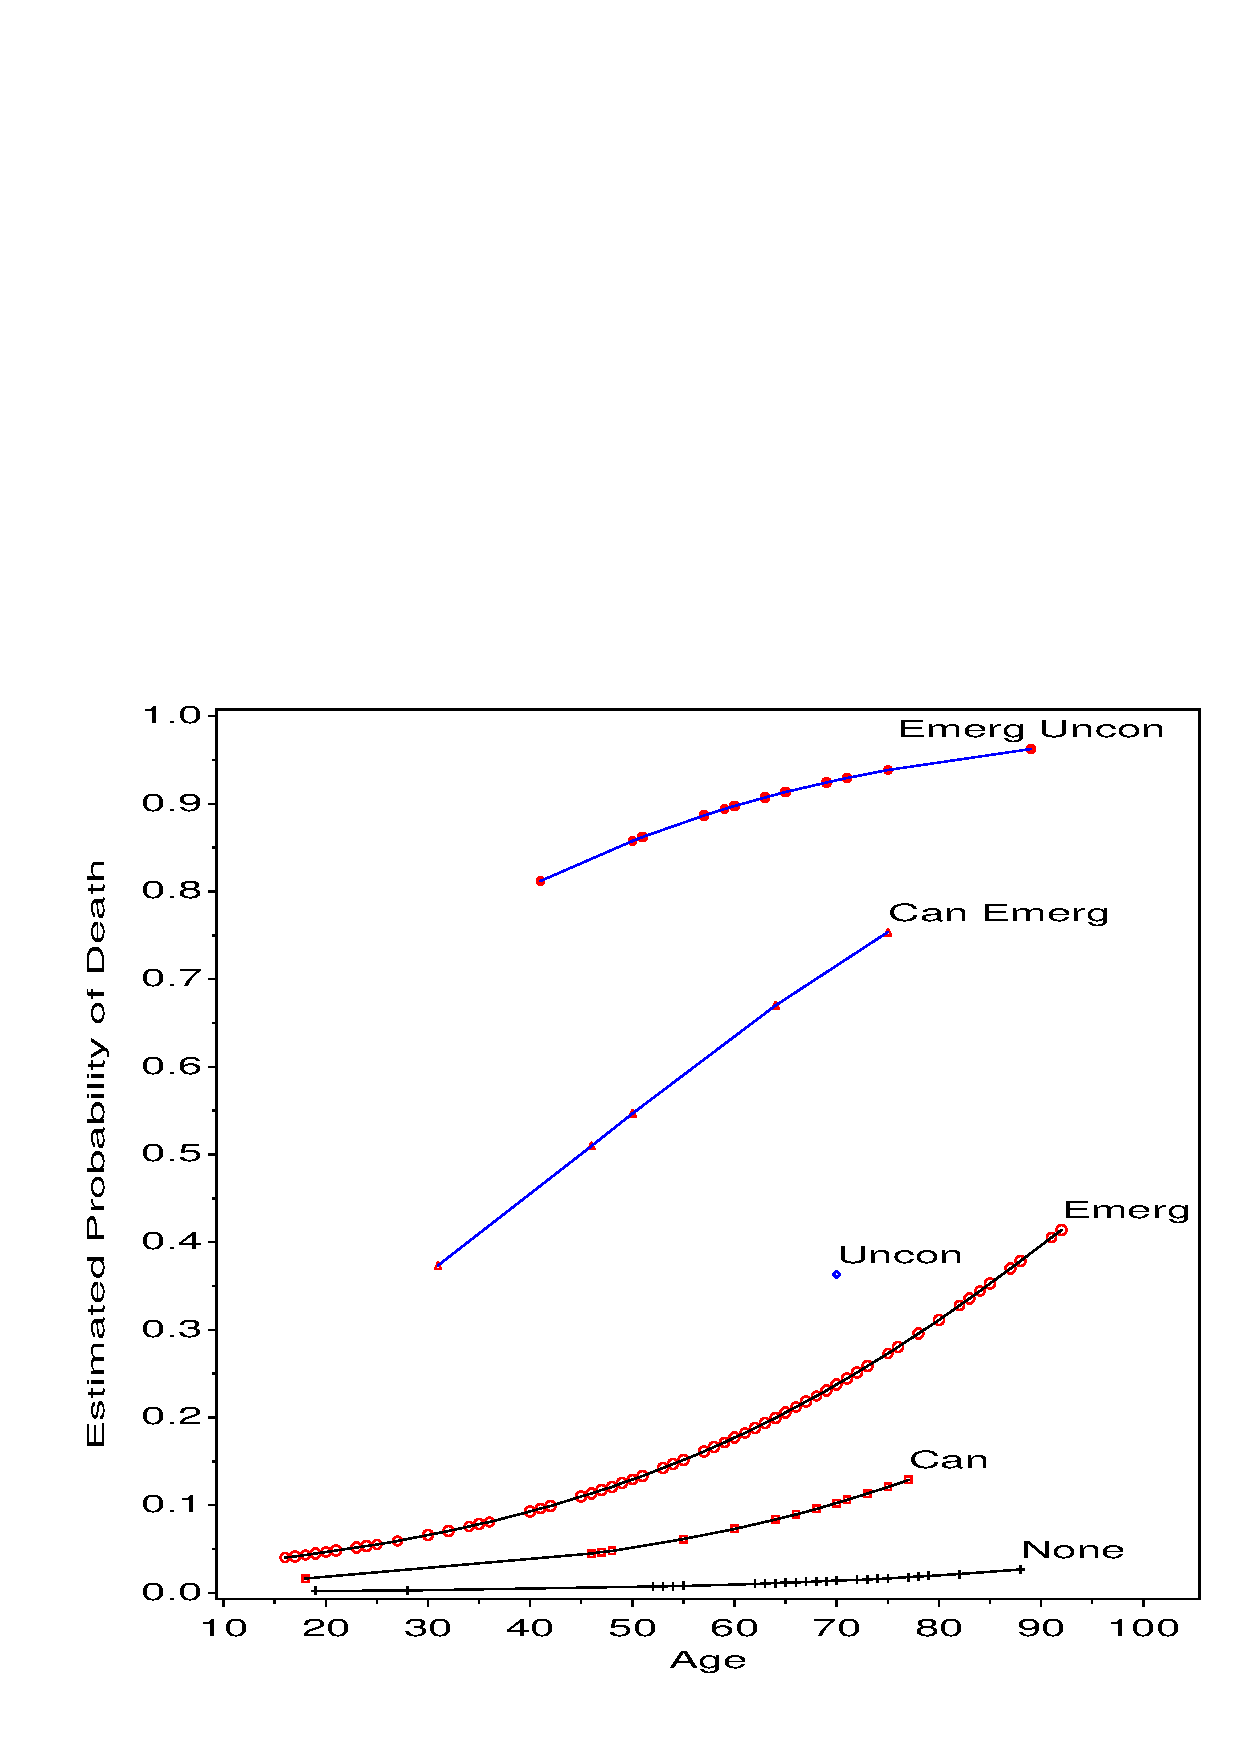
\includegraphics[scale=.6]{ch6/fig/icu11}
  \caption[ICU Survival data: Predicted probabilities]{ICU Survival data: Predicted probabilities for combinations of risk factors vs.\ age}%
  \label{fig:icu11}
\end{figure}
\begin{listing}
data label;
   set results;
   by risk;
   retain xsys ysys '2';
   position ='3';
   if predict>.9 then position='2';
   if last.risk then do;
      x = age;  y=predict;
      function = 'label   ';
      text=risk;
      output;
      end;

proc gplot data=results;
   plot predict * age = risk /
      frame anno=label vaxis=axis1 haxis=axis2 vm=1 hm=1 nolegend;
   axis1 label=(a=90);
   axis2 offset=(,4);
   symbol1 i=join v=square   c=red ci=black;
   symbol2 i=join v=triangle c=red ci=blue;
   symbol3 i=join v=circle   c=red ci=black;
   symbol4 i=join v=dot      c=red ci=blue;
   symbol5 i=join v=plus     c=black;
   symbol6 i=join v=diamond  c=blue ci=blue;
 run; quit;
\end{listing}
From the graph, it is apparent that mortality increases with
age when any of these risk factors are present, particularly
when the patient is admitted to Emergency; it is highest when the
patient is also unconscious at admission.  
From the odds ratios (see \outref{out:icu1.1}), we see that the
odds of death are increased 40-fold when the patient is unconscious.
The graph, however, shows the effects of these risk factors in
combination, and also indicates the number and age distribution of cases which have these combinations.

Before concluding that this model provides an adequate description of the
data, we should examine whether any individual cases are unduly influencing
the predicted results, and more importantly, the choice of variables in
the model.  We examine this question in \secref{sec:logist-infl}
where we return to these data (\exref{ex:icu2}).
\end{Example}

\subsection{Models with interaction}\label{sec:logist-multint}
The examples for the arthritis data have involved only main effects
of sex, age, and treatment.  We first illustrate tests for interactions
and powers of quantitative variables.
Whether interactions are present or not, the plotting of
estimated logits or predicted probabilities from \PROC{LOGISTIC} is no
more complicated in models with interactions.

In fact, since the predicted probabilities and logits are calculated
by the procedure and output to the \Dset\ \pname{RESULTS}, the results
plotted depend \emph{purely} on the \stmt{MODEL}{LOGISTIC}.  The plotting
steps remain the same as used in \figref{fig:glogist1b}, 
assuming you want to make separate plots for
males and females of the age by treatment effects.
For more complex models, or situations where you wish to plot predicted
results averaged over some variables, a method for plotting effects from
the model coefficients is described in \secref{sec:logistic-effplot}.

\begin{Example}[arthrit11]{Arthritis treatment}
The interaction effects were defined in the data step \pname{arthrit}
in \exref{ex:arthrit10} as
the dummy variables, \pname{agesex}, \pname{agetrt}, and \pname{sextrt}.  The
variable \pname{age2 = age**2} can be used to test whether the
relationship between age and logit(better) is quadratic rather than
linear.

A simple way to test for the need to include \emph{any} of these
more complex terms is illustrated here.
The \PROC{LOGISTIC} step below requests a forward-selection procedure.
Setting \pname{START=3} requests that the model building begin with the first
three variables (the main effects) listed in the model statement.
The option
\pname{SLENTRY=1} (significance level to enter) forces all variables to enter
the model eventually.

\begin{listing}
proc logistic data=arthrit;
   format better outcome.;
   model  better = _sex_ _treat_ age        /* main effects  */
                   agesex agetrt sextrt     /* interactions  */
                   age2                     /* quadratic age */
          / selection=forward
            start=3               /* start with main effects */
            slentry=1;           /* force all terms to enter */
\end{listing}

The variables included in each model for the selection procedure are
listed in a note at the beginning of each set of results:

\begin{output}
   Step  0. The following variables were entered:
            INTERCPT  _SEX_     _TREAT_   AGE
\end{output}

Results for this step are identical to those of the main effects
model given earlier.  Near the end of this step, the residual
\(\chi^2\) is printed, which corresponds to a joint test for the
other four variables.  This test is an appropriate test of goodness
of fit of the main effects model.

\begin{output}
   Residual Chi-Square = 4.0268 with 4 DF (p=0.4024)
\end{output}

Other tests printed show none of the interaction terms is significant
individually.
\end{Example}

\subsection{Effect plots from coefficients}\label{sec:logistic-effplot}
You can also construct plots for a fitted model
by calculating the predicted logit values directly from
the coefficients for the variables in the model.
This method can be used when raw data are not available, or when you
wish to average over certain effects to present simplified views of
a complex model.
To illustrate, for the arthritis
main effect model, the fitted relationship is
\begin{equation*}
  \logit ( p )  =
  - 4.5033  +
  1.4878 \,  \mbox{sex}   +
  1.7598 \,  \mbox{treat}  +
  0.0487 \,  \mbox{age}
  \period
\end{equation*}

With this method, the logit is calculated for each independent variable varied over its
range in all possible combinations.
Fixing an explanatory variable at its average gives an
effects plot for the remaining variables, which is particularly
useful when that
variable does not interact with others.
\citet{Fox:87} explains how this method may be used to construct adjusted
effects plots for particular interactions, adjusting for other
variables not represented in the plot.

The response can also be graphed on the probability scale by
transforming the logit via \(p = \exp(\logit) / ( 1  +  \exp(\logit) )\).  For example, the fitted logits and corresponding
probabilities for the arthritis data can be calculated in this data step:

\begin{listing}
data fitted;
  do _sex_ = 0 to 1;
     do _treat_ = 0 to 1;
        do age = 25 to 75 by 5;
           logit= -4.5033 + 1.4878*_sex_ + 1.7598*_treat_ + 0.0487*age;
           prob = exp(logit) / (1 + exp(logit));
           output;
           end;
        end;
     end;
\end{listing}
Replacing the outer \pname{DO}-loop with \verb|_sex_| = $\Pr_{\mbox{\scriptsize Female}} = 59/84 = .702$
would give fitted values at the average over sex; using \verb|_sex_| = 1/2
would give fitted values for a population with an equal sex distribution.

\begin{Example}[davis]{Volunteering for a psychological experiment}
\citet{Fox:87} illustrated this method using data from a study by \citet{CowlesDavis:87} on the personality factors which predispose
people to volunteer for a psychological experiment.
In this study, 1421 university students completed a personality inventory,
which contained a 24-item scale of Introversion-Extroversion
and a 24-item scale of Stability-Neuroticism, among other measures.
They were also asked to indicate their willingness in principle to
volunteer for a psychological experiment, which was the response to
be explained by the personality variables.

Fox reports the results of a logistic regression fit to these data
as
\begin{equation*}
\logit ( \pi_v ) = -2.605 + 0.2472 \mbox{ Sex} + 0.1668 E + 0.1108 N - 0.0088552 E \times N \quad ,
\end{equation*}
where $\pi_v$ is the probability of volunteering, Sex is a dummy variable
coded 0 for males and 1 for females, $E$ is the Introversion-Extroversion
score on a scale of 0--24, and $N$ is the Stability-Neuroticism score,
also on a scale of 0--24.

In this model, the positive coefficient for sex implies that women are
more likely to volunteer than men at each combination of extroversion
and neuroticism.
Because sex does not interact with either extroversion or neuroticism
we may focus on the relation between the probability of volunteering
and the two personality variables.
Setting \pname{sex=.5} in the \Dstp\ below generates observations
for the adjusted effects in a population equally composed of men and women.%
\footnote{Alternatively, we could set \pname{sex=0.55},
the proportion of women in the sample.}
\begin{listing}
data predict;
   array b\{0:4\} _temporary_ (-2.605  0.2472  0.1668  0.1108 -0.008552);
   do sex = 0 to 1 by .5;
      do neurot = 0 to 24 by 6;
         do extra = 0 to 24 by 6;
            logit = b[0] + b[1]*sex + b[2]*extra + b[3]*neurot
                  + b[4]*extra*neurot;
            prob = exp(logit) / ( 1 + exp(logit) );
            output;
            end;
         end;
      end;
\end{listing}

At a given level of sex, we may graph the fitted probability of volunteering
(\pname{prob}) against one predictor (say, extroversion) with separate
curves for each level of the other predictor (neuroticism).
The graph for the average over sex is shown in \figref{fig:davisn2}.
First, we may find the average probability of volunteering
by averaging the logits and transforming the average values to the
probability scale.
%% one figure
\begin{figure}[htb]
  \centering
  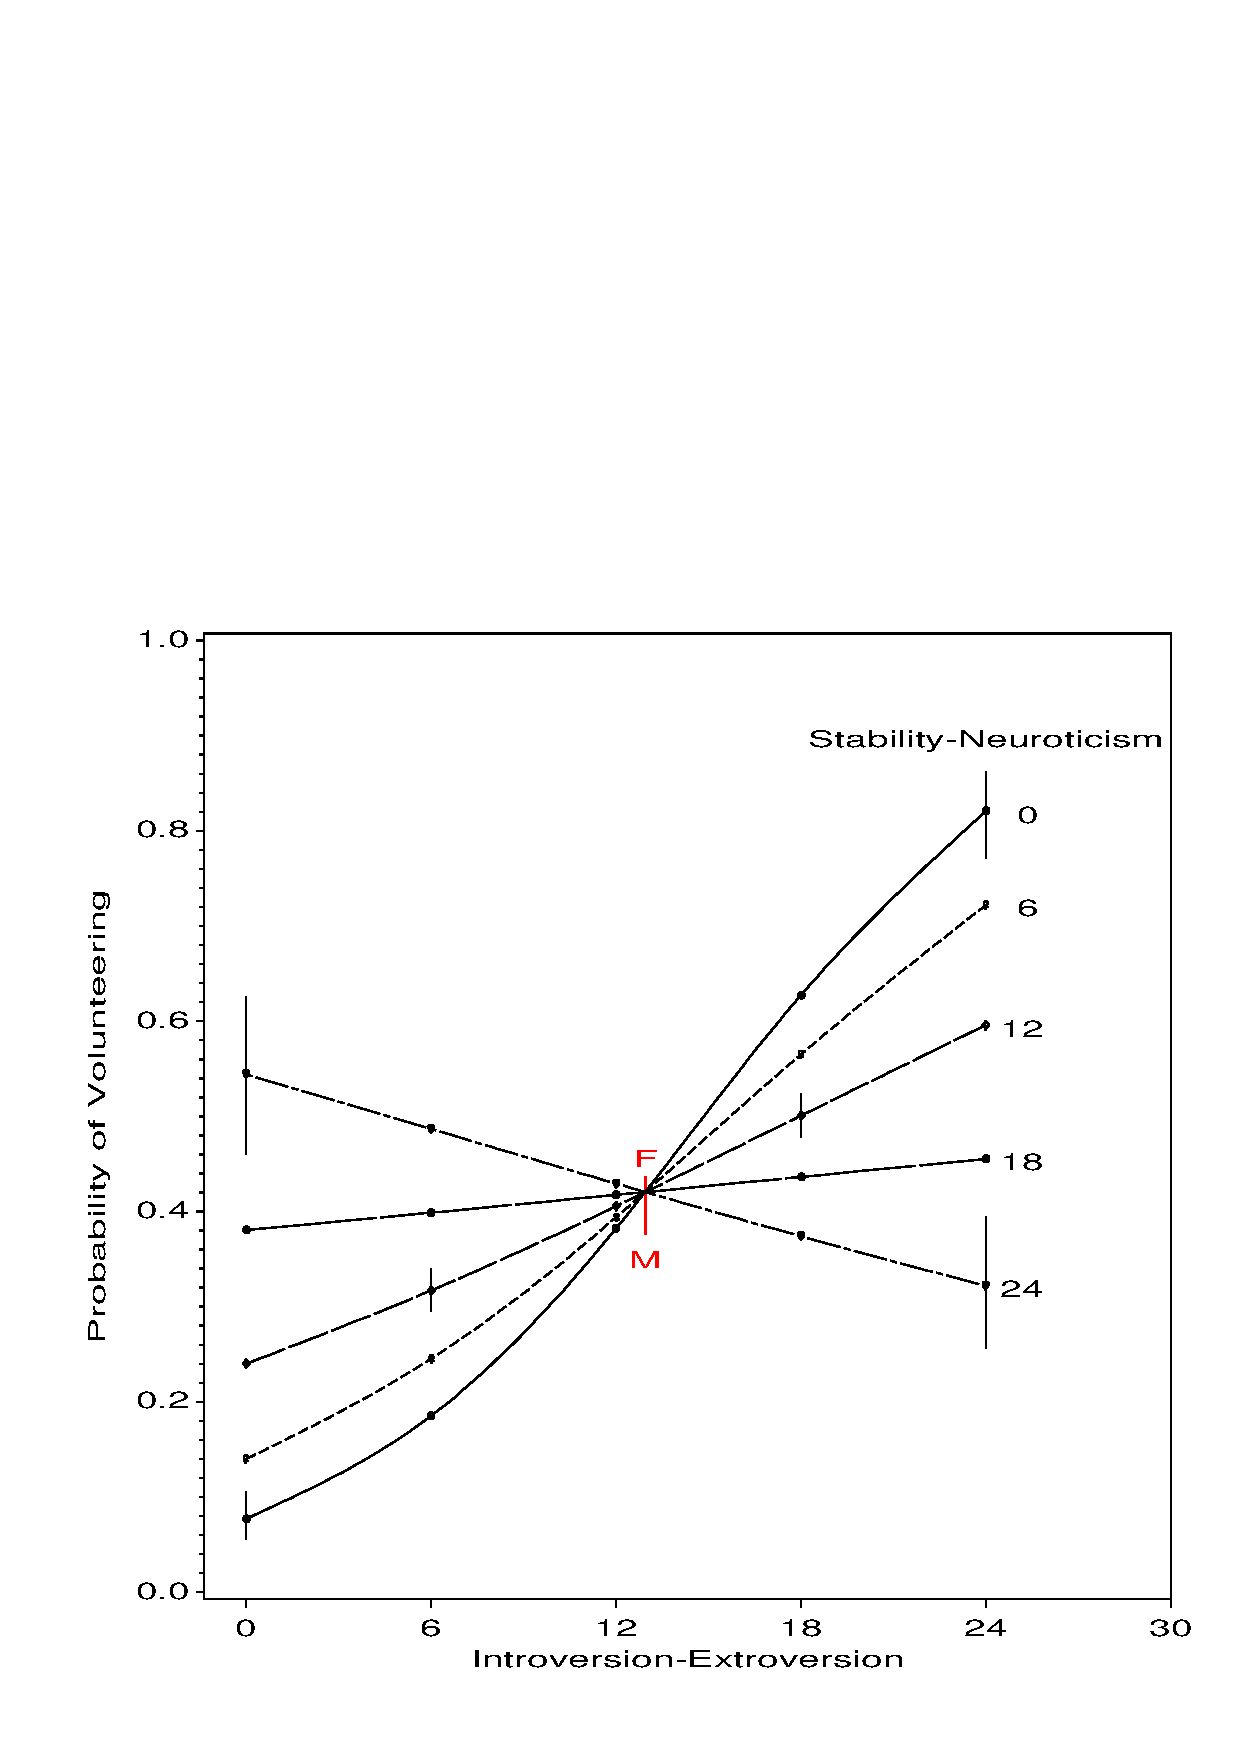
\includegraphics[scale=.6]{ch6/fig/davisn2}
  \caption[Fitted probability of volunteering, controlling for sex]{Fitted probability of volunteering, controlling for sex.  The effect of sex is shown
  at the point where the curves intersect.  The vertical lines at other
  selected combinations of extroversion and neuroticism show individual
  50\% confidence intervals.}%
  \label{fig:davisn2}
\end{figure}
\begin{listing}
proc summary nway data=predict;
   class sex;
   var logit ;
   output out=means mean=;
data means;
   set means;
   drop _type_ _freq_;
   prob = exp(logit) / (1 + exp(logit));
proc print;
\end{listing}
which gives
\begin{output}
                     OBS    SEX      LOGIT       PROB

                      1     0.0    -0.50587    0.37616
                      2     0.5    -0.38230    0.40557
                      3     1.0    -0.25872    0.43568
\end{output}
The statements below create an \ADS\ which supplies the labels
for the levels of neuroticism in the figure.
The effect of sex is shown by drawing a vertical line
showing the average probability of volunteering for men and for women
at the center of the graph.
\begin{listing}
proc format;
   value sex 0='Male'
            .5=' '           /* average */
             1='Female';
data anno;
   set predict;
   by sex neurot;
   xsys='2'; ysys='2';
   length text $22 function color $8;
   position='5';
   if last.neurot then do;
      x=extra+1;
      y=prob;
      text = put(neurot,3.0); function='LABEL'; output;
      end;

   if first.sex then do;
      y=.90;
      x=24; text='Stability-Neuroticism';
      function='LABEL'; output;
      x=2; text=put(sex,sex.);
      function='LABEL'; output;
      if text =' ' then do;
         color = 'red';
         x = 12.956;                * intersection of curves;
         y = 0.43568;               * average prob for females;
         function = 'MOVE '; output;
         text = 'F'; position = '2';
         function = 'LABEL' ; output;
         y = 0.37616;               * average prob for males;
         function = 'DRAW ' ; output;
         text = 'M'; position = '8';
         function = 'LABEL' ; output;
         end;
      end;
\end{listing}
The graph in \figref{fig:davisn2} is the second of three panels 
(for \pname{SEX=0.5}) drawn by the
\PROC{GPLOT} step below.
The other two graphs have the same form, shifted up for females
and down for males, as indicated by the vertical bar at the
intersection of the curves in \figref{fig:davisn2}.
\begin{listing}
goptions hby=0;
proc gplot data=predict;
   plot  prob * extra = neurot /
         vaxis=axis1 haxis=axis2 hminor=0
         frame nolegend anno=anno;
   by sex;
   axis1 label=(a=90) order=(0 to 1 by .2);
   axis2 label=(h=1.5 'Introversion-Extroversion')
         order=(0 to 30 by 6)  offset=(3,0);
   symbol1 v=+ i=spline l=1 c=black;
   symbol2 v=* i=spline l=3 c=black;
   symbol3 v=$ i=spline l=5 c=black;
   symbol4 v=- i=spline l=7 c=black;
   symbol5 v=# i=spline l=9 c=black;
\end{listing}
The interpretation of these results is quite clear from the graph.
At low levels of neuroticism, probability of volunteering increases
with extroversion, but the slope of this relation decreases
as neuroticism increases.
(If you want a lot of volunteers in a psychological experiment,
look for extraverted non-neurotics.)
At the highest levels of neuroticism,
probability of volunteering decreases with extroversion.

The error bars shown in \figref{fig:davisn2} require the estimated
variance-covariance matrix of the coefficients, $\widehat{\mathcal{V} (\vec{b})} = (\mat{X}\trans \mat{V} \mat{X})^{-1}$,
in addition to the coefficients themselves.
Because the fitted value, $\logit (\pi_i) = \vec{x}_i \trans \vec{b}$,
 is a linear combination of the parameters,
its standard error may be calculated as
\begin{equation*}
\mbox{s.e.} \logit (\pi_i) =
 [ \vec{x}_i \trans \widehat{\mathcal{V} (\vec{b})} \vec{x}_i ] ^ {1/2}
\end{equation*}
An approximate 50\% confidence interval for the fitted logit may
then be calculated as $\logit (\pi_i) \pm 0.67 \times \mbox{s.e.} \logit (\pi_i)$,
and the end points transformed back to the probability scale.

For example, the \Dstp\ below read the coefficients and the estimated
variance-covariance matrix in the form it would be produced by
\PROC{LOGISTIC} with the options \pname{OUTEST=PARMS COVOUT}
on the \pname{PROC} statement.
\begin{output}
data parms;
   input _type_ $ _name_ $ intercep sex extra neurot extneu;
datalines;
PARMS   ESTIMATE  -2.60551   0.24715   0.16682   0.11078  -.0085525
COV     INTERCPT   0.27504  -0.01839  -0.01819  -0.01726  0.0012943
COV     SEX       -0.01839   0.01246   0.00013  -0.00007  -.0000134
COV     INTEXT    -0.01819   0.00013   0.00142   0.00127  -.0001023
COV     NEUROT    -0.01726  -0.00007   0.00127   0.00142  -.0001052
COV     EXTNEU     0.00129  -0.00001  -0.00010  -0.00011  0.0000086
;
\end{output}
(If this analysis was carried out using raw data, the \pname{OUTEST=PARMS}
\Dset\ could be used directly.)
Calculation of the standard errors and confidence intervals is
then done most easily with \IML, as follows:
%\begin{changebar}
\begin{listing}
proc iml;
   use parms;
   read var\{intercep sex extra neurot extneu\} into b where(_type_='PARMS');
   read all var\{intercep sex extra neurot extneu\} into cov
       where(_type_='COV');
   b = t(b);
   do sex = 0 to 1 by .5;
      do neurot = 0 to 24 by 6;
         do extra = 0 to 24 by 6;
            x = 1 || sex || extra || neurot || extra#neurot;
            logit = x * b;
            selogit = sqrt( x * cov * t(x) );
            prob = exp(logit) / ( 1 + exp(logit) );
            result = result // ( x[,2:4] || logit || selogit || prob );
            end;
         end;
      end;
  ul = result[,4] + .67#result[,5];
  ll = result[,4] - .67#result[,5];
  lower = exp(ll) / ( 1 + exp(ll) );
  upper = exp(ul) / ( 1 + exp(ul) );
  var = \{sex extra neurot logit selogit prob lower upper\};
  result = result || lower || upper;
  create predict from result[c=var];
  append from result;
quit;
\end{listing}
%\end{changebar}
The error bars in \figref{fig:davisn2} serve notice that the predicted
probabilities are most precise for those with average levels of
the explanatory variables, as is usual with linear models.
\end{Example}
